\documentclass[aspectratio=169]{beamer}
\usetheme{Madrid}
\usecolortheme{default}
\usepackage{booktabs}
\usepackage{graphicx}
\usepackage{tikz}
\usepackage{multicol}
\usepackage{listings}
\usetikzlibrary{arrows.meta, positioning}

% Wayne State University Colors
\definecolor{wsugreen}{RGB}{12, 84, 73}
\definecolor{wsugold}{RGB}{255, 206, 0}
\definecolor{wsudarkgold}{RGB}{197, 169, 0}
\definecolor{wsulightgreen}{RGB}{220, 237, 234}

\setbeamercolor{title}{fg=white, bg=wsugreen}
\setbeamercolor{frametitle}{fg=white, bg=wsugreen}
\setbeamercolor{structure}{fg=wsugreen}
\setbeamercolor{block title}{bg=wsugreen!15, fg=wsugreen}
\setbeamercolor{block body}{bg=wsugreen!5}
\setbeamercolor{item}{fg=wsugreen}
\setbeamercolor{footline}{fg=wsugreen, bg=wsugreen!10}
\setbeamercolor{title in head/foot}{fg=white, bg=wsugreen}
\setbeamercolor{author in head/foot}{fg=wsugreen, bg=wsugreen!10}
\setbeamercolor{date in head/foot}{fg=wsugreen, bg=wsugreen!10}

\lstdefinelanguage{Solidity}{
  keywords={pragma, solidity, contract, function, modifier, require, returns, return, mapping, address, uint, uint256, bool, string, public, private, internal, external, view, pure, payable, memory, if, else, emit, event, msg, block, this},
  morecomment=[l]{//},
  morecomment=[s]{/*}{*/},
  morestring=[b]",
  sensitive=true,
}
\lstset{
  basicstyle=\tiny\ttfamily,
  breaklines=true,
  frame=single,
  numbers=left,
  numberstyle=\tiny\color{gray},
  keywordstyle=\bfseries\color{wsugreen},
  commentstyle=\itshape\color{gray},
  tabsize=2,
}

\title[LLM Smart Contract Security]{From Prompt to Exploit:\\Security Vulnerabilities in LLM-Generated Smart Contracts}
\subtitle{CSC 5991 --- Final Project Presentation}
\author{Anik Tahabilder \and Dong Vo}
\institute{Wayne State University}
\date{April 21, 2026}

\begin{document}

%--- Slide 1: Title ---
\begin{frame}
\titlepage
\end{frame}

%--- Slide 2: Outline ---
\begin{frame}{Outline}
\begin{enumerate}
    \item Background on Smart Contracts
    \item Motivation
    \item Research Questions
    \item Methodology
    \item Results (RQ1--RQ4)
    \item Root Cause Analysis
    \item Human Review
    \item Mitigation and Proposed Pipeline
    \item Conclusions
\end{enumerate}
\end{frame}

%--- Slide 3: Background ---
\begin{frame}{Background: Smart Contracts}
\begin{columns}
\begin{column}{0.55\textwidth}
\begin{itemize}
    \item Programs on the blockchain (mostly Ethereum)
    \item Written in Solidity
    \item Power DeFi, NFTs, DAOs, bridges
    \item Hold \textbf{hundreds of billions of dollars}
\end{itemize}
\end{column}
\begin{column}{0.42\textwidth}
\textbf{Three key properties:}
\begin{itemize}
    \item \textbf{Immutable} --- can't be patched
    \item \textbf{Public} --- anyone can read the code
    \item \textbf{Adversarial} --- anyone can call it
\end{itemize}

\vspace{0.25cm}
\begin{block}{}
\centering One bug $\to$ instant exploit.
\end{block}
\end{column}
\end{columns}
\end{frame}

%--- Slide 4: Motivation ---
\begin{frame}{Motivation}
\begin{columns}
\begin{column}{0.55\textwidth}
\begin{itemize}
    \item Developers use ChatGPT, Copilot, Claude to write Solidity
    \item \$3.8B stolen from smart contract bugs in 2022
    \item Once deployed --- \textbf{no patches}
    \item Perry et al.\ (CCS 2023): AI users write less secure code but \textbf{feel safer}
    \item Nobody has measured this at scale
\end{itemize}
\end{column}
\begin{column}{0.4\textwidth}
\centering
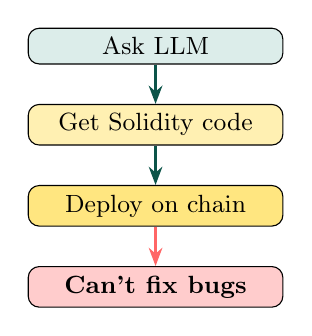
\begin{tikzpicture}[scale=0.85]
    \node[draw, rounded corners, fill=wsulightgreen, text width=3cm, align=center, font=\small] (dev) {Ask LLM};
    \node[draw, rounded corners, fill=wsugold!30, text width=3cm, align=center, font=\small, below=0.5cm of dev] (code) {Get Solidity code};
    \node[draw, rounded corners, fill=wsugold!50, text width=3cm, align=center, font=\small, below=0.5cm of code] (deploy) {Deploy on chain};
    \node[draw, rounded corners, fill=red!20, text width=3cm, align=center, font=\small\bfseries, below=0.5cm of deploy] (vuln) {Can't fix bugs};
    \draw[-{Stealth}, thick, wsugreen] (dev) -- (code);
    \draw[-{Stealth}, thick, wsugreen] (code) -- (deploy);
    \draw[-{Stealth}, thick, red!60] (deploy) -- (vuln);
\end{tikzpicture}
\end{column}
\end{columns}
\end{frame}

%--- Slide 5: Research Questions ---
\begin{frame}{Research Questions}
\vspace{0.3cm}
\begin{itemize}
    \item[\textbf{RQ1.}] How common are bugs? Do LLMs differ?
    \vspace{0.4cm}
    \item[\textbf{RQ2.}] What kinds of bugs? Any LLM-specific patterns?
    \vspace{0.4cm}
    \item[\textbf{RQ3.}] Do tricky prompts make it worse?
    \vspace{0.4cm}
    \item[\textbf{RQ4.}] How does LLM code compare to real Ethereum code?
\end{itemize}
\end{frame}

%--- Slide 6: Methodology ---
\begin{frame}{Methodology and Dataset}
\begin{center}
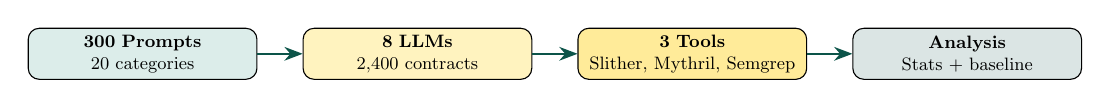
\begin{tikzpicture}[node distance=0.6cm, scale=0.72, transform shape]
    \node[draw, rounded corners, fill=wsulightgreen, text width=3.8cm, align=center, font=\small, minimum height=0.9cm] (p1) {\textbf{300 Prompts}\\20 categories};
    \node[draw, rounded corners, fill=wsugold!25, text width=3.8cm, align=center, font=\small, minimum height=0.9cm, right=0.8cm of p1] (p2) {\textbf{8 LLMs}\\2,400 contracts};
    \node[draw, rounded corners, fill=wsugold!40, text width=3.8cm, align=center, font=\small, minimum height=0.9cm, right=0.8cm of p2] (p3) {\textbf{3 Tools}\\Slither, Mythril, Semgrep};
    \node[draw, rounded corners, fill=wsugreen!15, text width=3.8cm, align=center, font=\small, minimum height=0.9cm, right=0.8cm of p3] (p4) {\textbf{Analysis}\\Stats $+$ baseline};
    \draw[-{Stealth}, thick, wsugreen] (p1) -- (p2);
    \draw[-{Stealth}, thick, wsugreen] (p2) -- (p3);
    \draw[-{Stealth}, thick, wsugreen] (p3) -- (p4);
\end{tikzpicture}
\end{center}

\vspace{0.3cm}
\begin{columns}
\begin{column}{0.5\textwidth}
\small
\textbf{General LLMs:} GPT-4o, GPT-5, Claude 3.5 Sonnet, Gemini 2.5

\textbf{Code LLMs:} DeepSeek, Qwen 2.5, CodeLlama, Codestral
\end{column}
\begin{column}{0.48\textwidth}
\small
\textbf{Baseline:} 241 real contracts from Etherscan (Uniswap, Aave, Compound, Lido, \ldots)
\end{column}
\end{columns}

\vspace{0.3cm}
\begin{block}{}
\centering\textbf{2,493 unique bugs} across 1,566 compiled contracts
\end{block}
\end{frame}

%--- Slide 7: RQ1 Prevalence ---
\begin{frame}{RQ1: Vulnerability Prevalence}
\begin{columns}
\begin{column}{0.42\textwidth}
\begin{center}
\footnotesize
\begin{tabular}{@{}lrr@{}}
\toprule
\textbf{Severity} & \textbf{Count} & \textbf{Contracts} \\
\midrule
High & 804 & 419 (26.8\%) \\
Medium & 619 & 397 (25.4\%) \\
Low & 987 & 584 (37.3\%) \\
\midrule
\textbf{Total} & \textbf{2,410} & \textbf{856 (54.7\%)} \\
\bottomrule
\end{tabular}
\end{center}

\vspace{0.2cm}
\begin{itemize}\small
    \item \textbf{Half} of contracts buggy
    \item \textbf{1 in 4} high-severity
\end{itemize}
\end{column}
\begin{column}{0.56\textwidth}
\centering
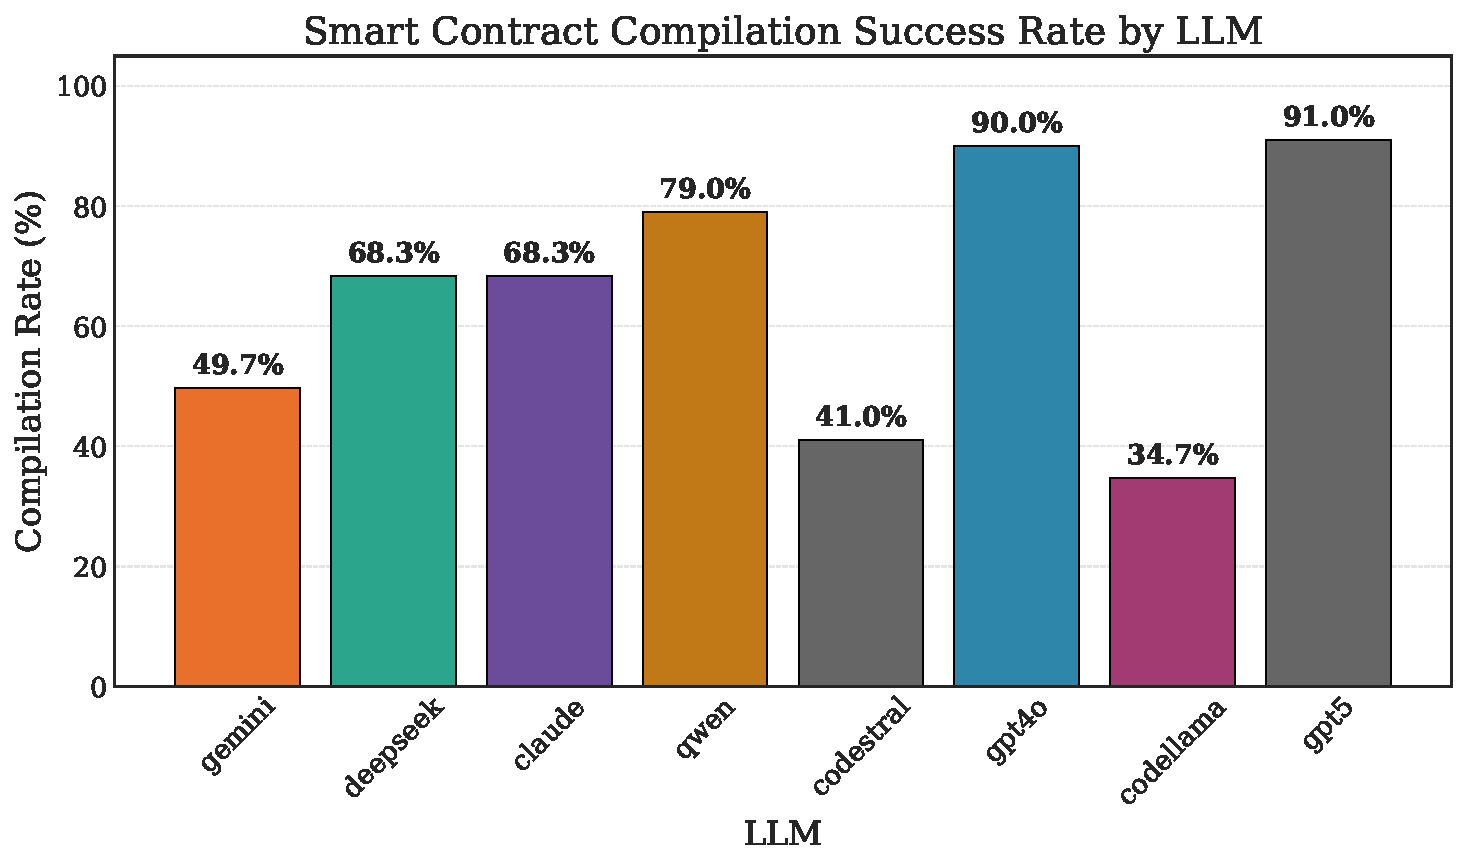
\includegraphics[height=0.30\textheight,keepaspectratio]{../visualization/figures/fig10_compilation_rates.pdf}\\[-0.05cm]
{\scriptsize Compile rates: 35\%--91\%}\\[0.15cm]
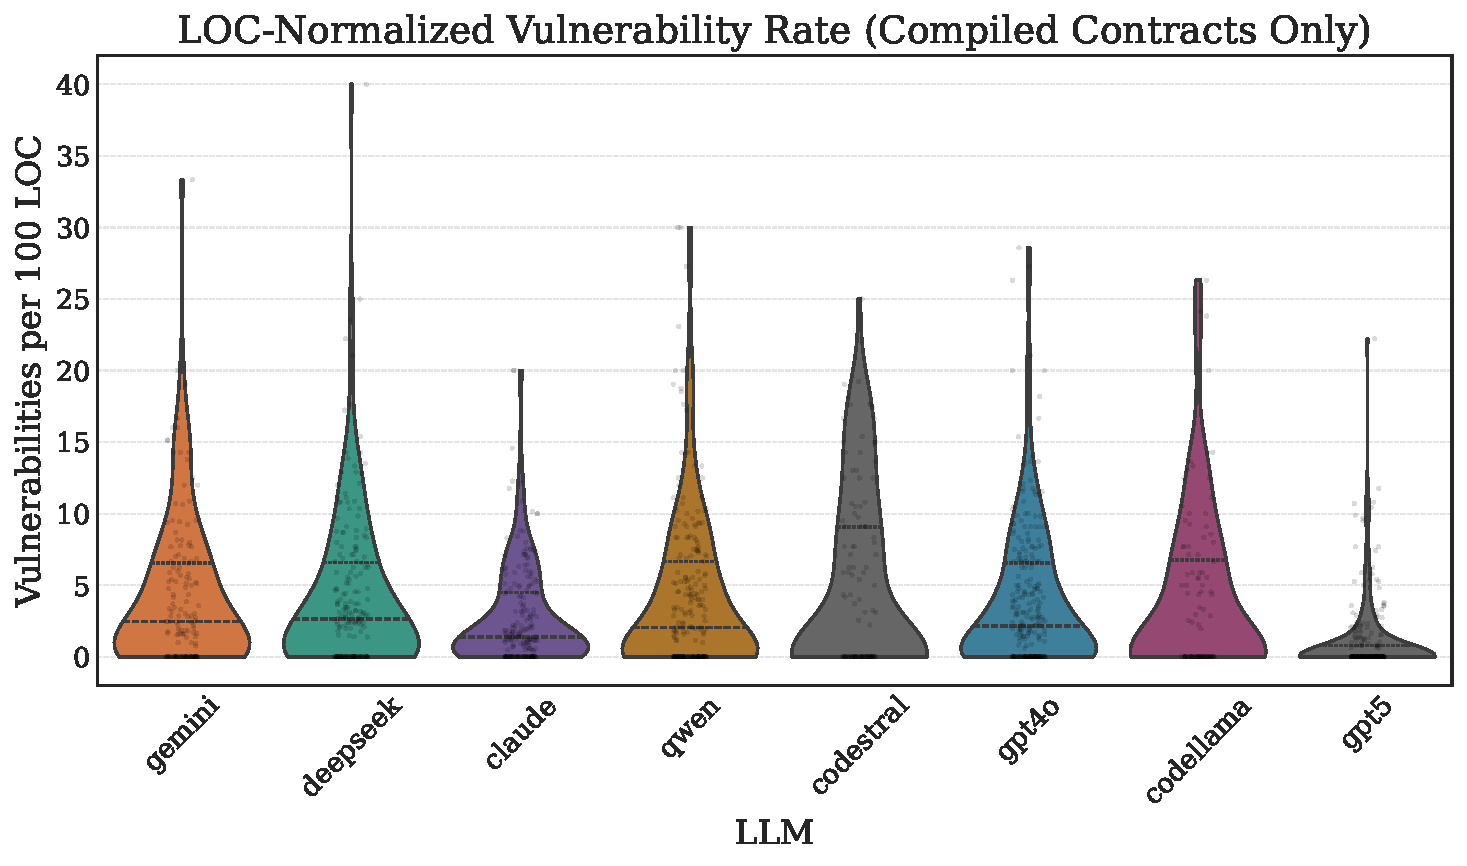
\includegraphics[height=0.30\textheight,keepaspectratio]{../visualization/figures/fig8_loc_normalized_violin.pdf}\\[-0.05cm]
{\scriptsize Bug density per 100 LOC}
\end{column}
\end{columns}
\end{frame}

%--- Slide 8: RQ1 Cross-LLM ---
\begin{frame}{RQ1: Cross-LLM Comparison}
\begin{center}
\scriptsize
\begin{tabular}{@{}llccccc@{}}
\toprule
\textbf{Model} & \textbf{Type} & \textbf{Compiles} & \textbf{\% Vuln} & \textbf{Mean Bugs} & \textbf{Bugs/100 LOC} & \textbf{Avg LOC} \\
\midrule
GPT-5               & General & \textbf{91.0\%} & 26.7\% & 0.63 & \textbf{0.99} & 49 \\
GPT-4o              & General & 90.0\% & 62.2\% & 1.65 & 3.86 & 52 \\
Qwen 2.5 Coder      & Code    & 79.0\% & 58.2\% & 1.40 & 4.10 & 42 \\
Claude 3.5 Sonnet   & General & 68.3\% & 69.3\% & 3.22 & 2.75 & 113 \\
DeepSeek Coder V2   & Code    & 68.3\% & 62.0\% & 1.44 & 4.24 & 38 \\
Gemini Flash-Lite   & General & 49.7\% & 66.4\% & 1.85 & 4.25 & 55 \\
Codestral 22B       & Code    & 41.0\% & 48.0\% & 1.06 & \textbf{4.88} & 24 \\
CodeLlama-34B       & Code    & 34.7\% & 48.1\% & 0.95 & 4.09 & 26 \\
\bottomrule
\end{tabular}
\end{center}

\vspace{0.3cm}
\begin{itemize}
    \item Big differences: Kruskal-Wallis $H = 132.7$, $p < 10^{-25}$
    \item \textbf{GPT-5 wins} --- best compile, lowest density
    \item General vs.\ code-specialized --- no clear winner per LOC
\end{itemize}
\end{frame}

%--- Slide 9: RQ2 Taxonomy ---
\begin{frame}{RQ2: Vulnerability Taxonomy}
\begin{columns}
\begin{column}{0.45\textwidth}
\small
\begin{tabular}{@{}rlr@{}}
\toprule
\textbf{\#} & \textbf{Type} & \textbf{Count} \\
\midrule
1 & Unchecked Return & 461 \\
2 & Reentrancy & 346 \\
3 & Access Control & 173 \\
4 & Coding Standards & 147 \\
5 & Incorrect Calc. & 85 \\
6 & Timestamp Dep. & 52 \\
7 & Uninitialized State & 35 \\
\bottomrule
\end{tabular}

\vspace{0.3cm}
\begin{itemize}\small
    \item Top 2: unchecked returns, reentrancy
    \item \textbf{All 8 LLMs share the same top CWEs}
\end{itemize}
\end{column}
\begin{column}{0.52\textwidth}
\centering
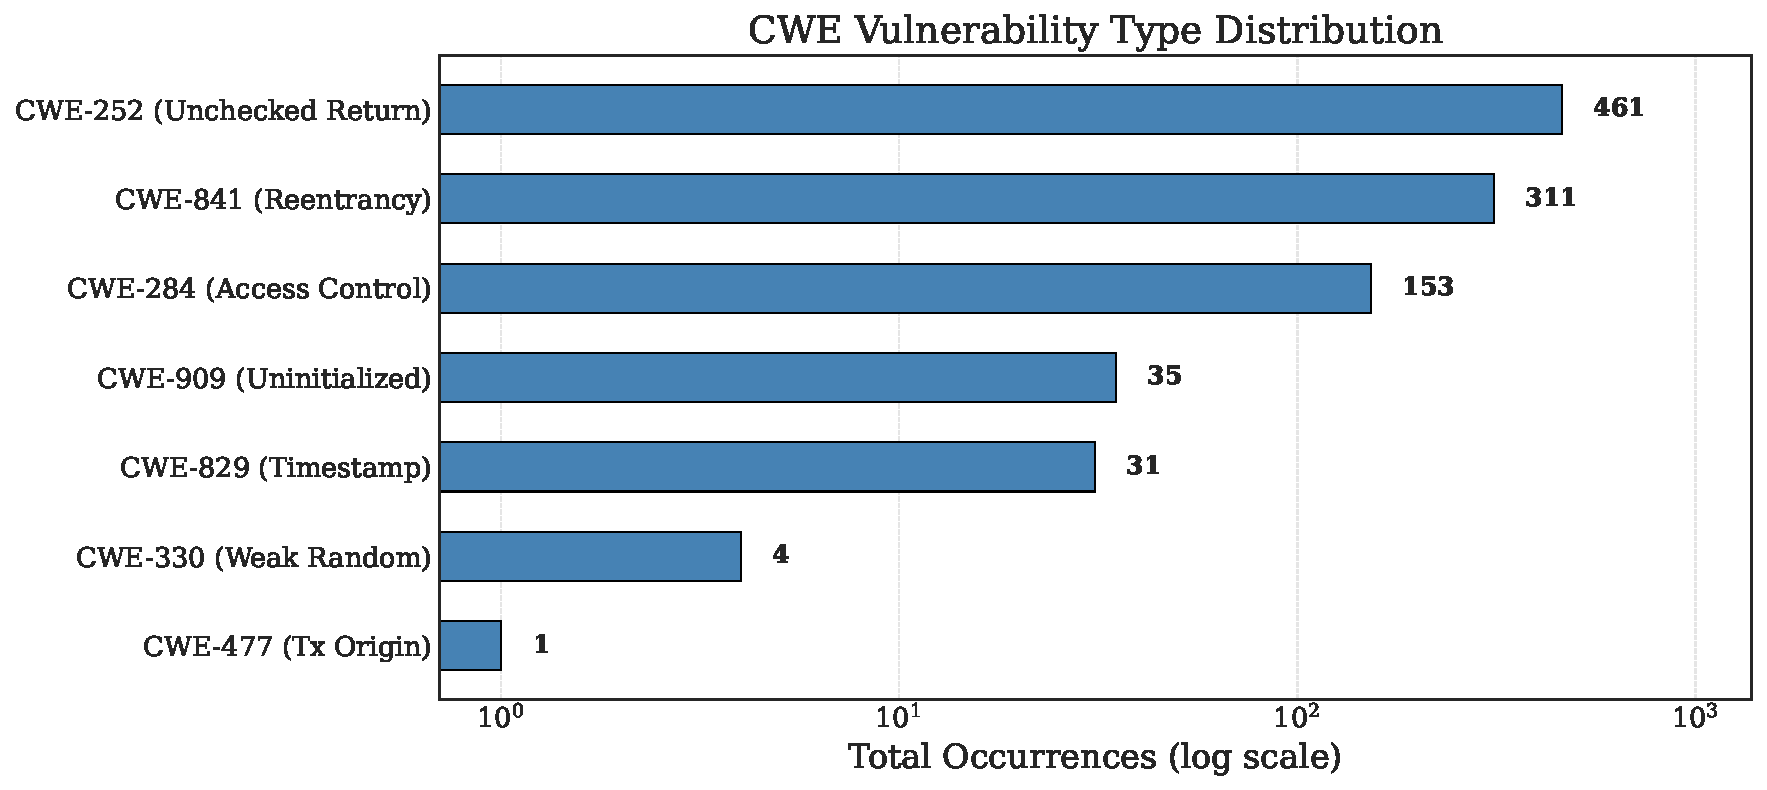
\includegraphics[width=\textwidth]{../visualization/figures/fig6_cwe_distribution.pdf}
\end{column}
\end{columns}
\end{frame}

%--- Slide 10: RQ2 Patterns ---
\begin{frame}[fragile]{RQ2: LLM-Specific Patterns}
\begin{columns}
\begin{column}{0.52\textwidth}

\textbf{1. Phantom Guards}\\
\small Empty \texttt{nonReentrant} --- looks safe, isn't.

\vspace{0.3cm}
\textbf{2. Unnecessary Reimplementations}\\
\small SafeMath on Solidity 0.8+ (4\% of contracts). DeepSeek worst.

\vspace{0.3cm}
\textbf{3. Context Window Degradation}\\
\small In long contracts, \textbf{4.1$\times$ more} risky code in the second half.

\end{column}
\begin{column}{0.46\textwidth}
\begin{lstlisting}[language=Solidity, caption={Phantom guard}]
// LLM-generated (VULNERABLE)
modifier nonReentrant() {
    _; // No lock!
}

function withdraw(uint amt)
    nonReentrant {
    payable(msg.sender)
      .call{value: amt}("");
    balances[msg.sender] -= amt;
}
\end{lstlisting}
\end{column}
\end{columns}
\end{frame}

%--- Slide 11: RQ3 Adversarial ---
\begin{frame}{RQ3: Adversarial Prompt Robustness}
\begin{columns}
\begin{column}{0.48\textwidth}
\centering
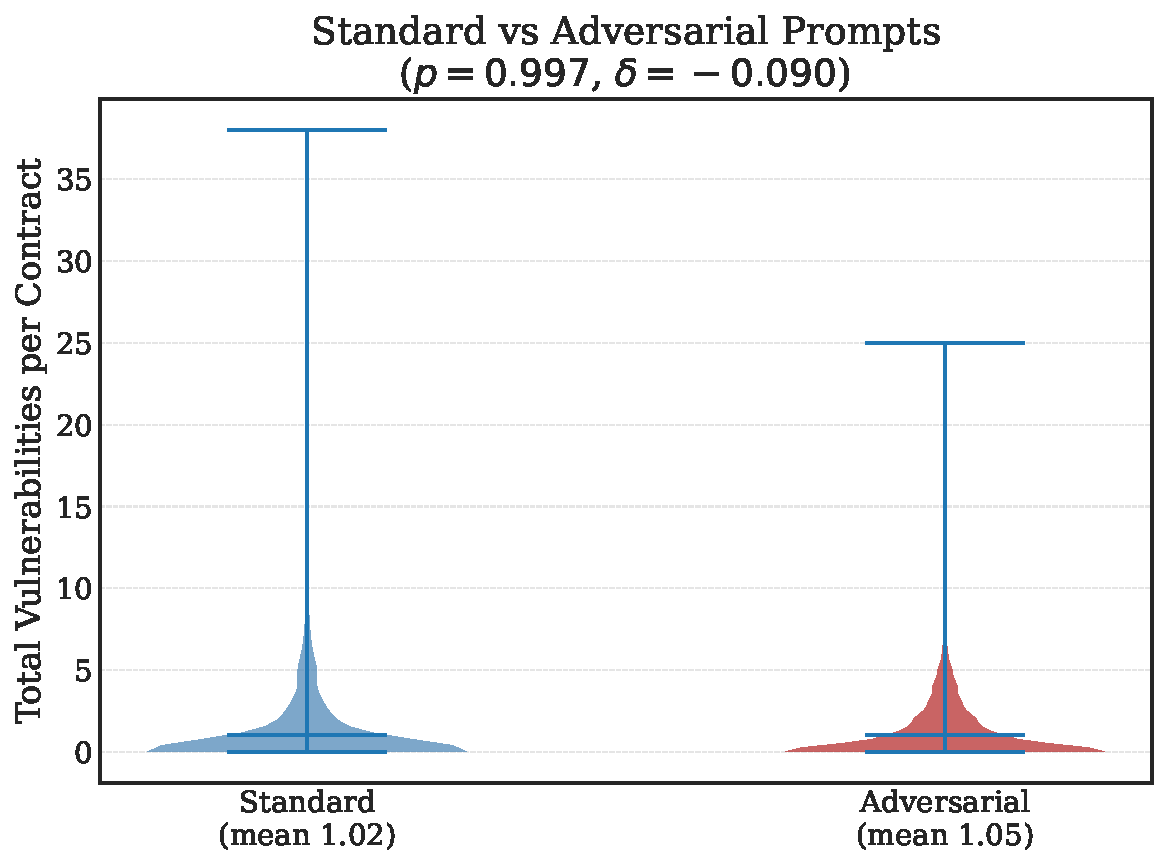
\includegraphics[width=\textwidth]{../visualization/figures/fig2_standard_vs_adversarial.pdf}
\end{column}
\begin{column}{0.48\textwidth}
\textbf{Short answer: No.}

\vspace{0.3cm}
\begin{itemize}\small
    \item $p = 0.965$ (not significant)
    \item Cliff's $\delta = -0.056$ (negligible)
    \item Adversarial $\approx$ standard
\end{itemize}

\vspace{0.3cm}
``Optimize gas,'' ``keep it minimal,'' ``no dependencies'' --- none hurt security.
\end{column}
\end{columns}

\vspace{0.2cm}
\begin{block}{Key insight}
\centering Bugs come from \textbf{training data}, not prompts. You can't prompt your way to safe code.
\end{block}
\end{frame}

%--- Slide 12: RQ4 Human Comparison ---
\begin{frame}{RQ4: LLM vs.\ Human-Written Contracts}
\begin{columns}
\begin{column}{0.46\textwidth}
\begin{center}
\small
\begin{tabular}{@{}lcc@{}}
\toprule
\textbf{Metric} & \textbf{Human} & \textbf{LLM} \\
\midrule
Contracts & 241 & 2,400 \\
Compiled & 54.8\% & 65.2\% \\
\% with bugs & 82.6\% & 54.7\% \\
Mean LOC & 446.7 & 52.3 \\
\textbf{Bugs/100 LOC} & \textbf{2.69} & \textbf{0.99--4.88} \\
High-sev \% & 16.0\% & 15.7\% \\
\bottomrule
\end{tabular}
\end{center}
\vspace{0.2cm}
\scriptsize Human: Uniswap, Aave, Compound, Gnosis, Lido
\end{column}
\begin{column}{0.5\textwidth}
\begin{itemize}\small
    \item Bug density \textbf{similar} per LOC
    \item High-severity rates \textbf{almost identical}
    \item Human contracts \textbf{8$\times$ larger}
\end{itemize}

\vspace{0.3cm}
\textbf{But:}
\begin{itemize}\small
    \item Human code was audited, tested, bountied, monitored
    \item LLM code usually just ships
\end{itemize}

\vspace{0.2cm}
\begin{block}{}
\centering The danger is \textbf{skipping the pipeline}.
\end{block}
\end{column}
\end{columns}
\end{frame}

%--- Slide 13: Root Cause ---
\begin{frame}{Root Cause Analysis}
\begin{columns}
\begin{column}{0.48\textwidth}
\textbf{1. Training data bias}
\begin{itemize}\small
    \item All 8 LLMs share top CWEs
    \item Trained on pre-2023 Solidity
    \item Adversarial null $\to$ \textbf{intrinsic}
\end{itemize}

\vspace{0.3cm}
\textbf{2. Compilation failures}
\begin{itemize}\small
    \item Bad \texttt{@openzeppelin} imports
    \item Markdown in code
    \item CodeLlama: 65\% syntax fails
\end{itemize}
\end{column}
\begin{column}{0.48\textwidth}
\textbf{3. Model fingerprints}
\begin{itemize}\small
    \item Claude: equality checks
    \item CodeLlama: bad ERC-20
    \item All: missing zero checks
\end{itemize}

\vspace{0.3cm}
\textbf{4. Category matters}
\begin{itemize}\small
    \item Worst: Proxy, Yield, DEX
    \item Safest: Access Control, ERC-20
\end{itemize}
\end{column}
\end{columns}
\end{frame}

%--- Slide 14: Human Review ---
\begin{frame}{Human Review Validation}
\begin{columns}
\begin{column}{0.48\textwidth}
\small
We manually reviewed 195 of the 241 baseline contracts.

\vspace{0.3cm}
\begin{tabular}{@{}lr@{}}
\toprule
\textbf{Metric} & \textbf{Result} \\
\midrule
Reviewed & 195 \\
With issues & 161 (82.6\%) \\
Total issues & 310 \\
High severity & 117 (37.7\%) \\
Medium severity & 163 (52.6\%) \\
\bottomrule
\end{tabular}
\end{column}
\begin{column}{0.48\textwidth}
\textbf{Top issues:}
\begin{enumerate}\small
    \item Access Control (72)
    \item Unchecked Returns (67)
    \item Integer Overflow (16)
    \item Reentrancy (16)
    \item External Calls (14)
\end{enumerate}

\vspace{0.3cm}
\textbf{Humans catch what Slither misses:} signature replay, centralization, storage collision.
\end{column}
\end{columns}

\vspace{0.2cm}
\begin{block}{}
\centering Tools $+$ humans $>$ tools alone.
\end{block}
\end{frame}

%--- Slide 15: Mitigation Attempt ---
\begin{frame}{Mitigation: Can a Security Prompt Fix It?}
\begin{columns}
\begin{column}{0.48\textwidth}
\textbf{What we tried:}\\
Add a ``use checks-effects-interactions, validate inputs, ReentrancyGuard, SafeERC20, \ldots'' preamble to 20 prompts (Claude).

\vspace{0.3cm}
\textbf{Hypothesis:} explicit security cues help.

\vspace{0.3cm}
\textbf{Result:} they don't.
\end{column}
\begin{column}{0.48\textwidth}
\begin{center}
\small
\begin{tabular}{@{}lrr@{}}
\toprule
\textbf{Metric} & \textbf{Plain} & \textbf{Prefix} \\
\midrule
Mean bugs & 2.20 & \textbf{8.73} \\
Got worse & \multicolumn{2}{c}{13 / 20} \\
Got better & \multicolumn{2}{c}{5 / 20} \\
\bottomrule
\end{tabular}
\end{center}

\vspace{0.3cm}
\textbf{Why:} prefix adds more code $\to$ more findings (mostly low-severity).

High-severity bugs actually went \textbf{down by 2}.
\end{column}
\end{columns}

\vspace{0.15cm}
\begin{block}{Takeaway}
\centering Prompts aren't the fix. The \textbf{pipeline} is.
\end{block}
\end{frame}

%--- Slide 16: Tool Agreement ---
\begin{frame}{No Single Tool Catches Every Bug}
\textit{\small Prompts can't fix the code (slide 15). So we need stronger detection --- but can one tool do it?}

\vspace{0.15cm}
\begin{columns}
\begin{column}{0.54\textwidth}
\centering
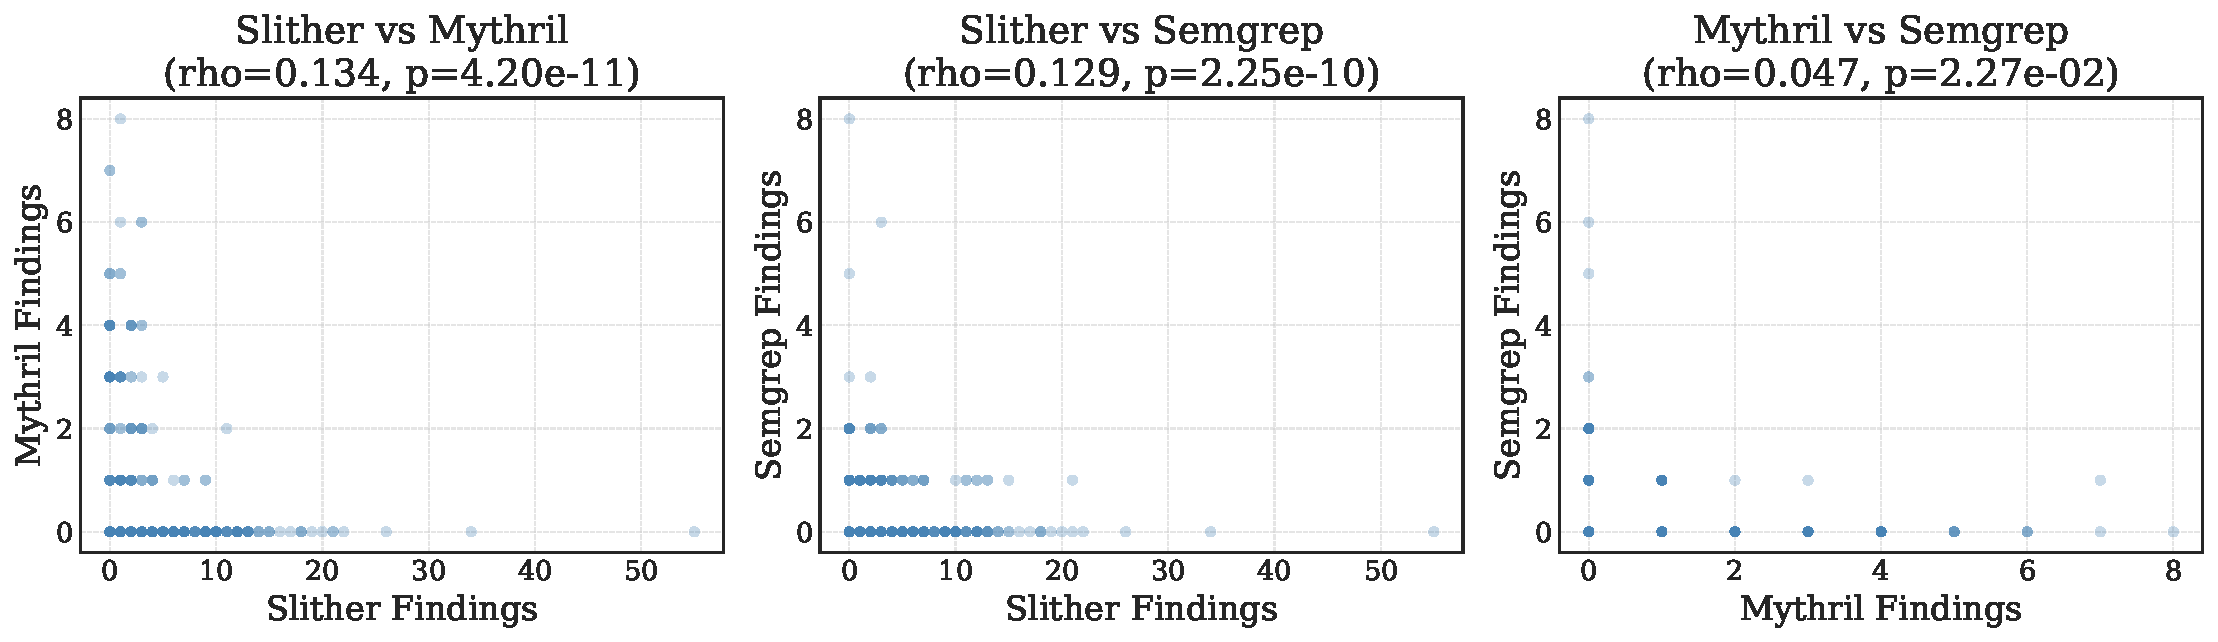
\includegraphics[width=\textwidth,keepaspectratio]{../visualization/figures/fig7_tool_agreement.pdf}
\end{column}
\begin{column}{0.44\textwidth}
\textbf{Agreement between the 3 analyzers (Spearman $\rho$):}
\begin{center}
\small
\begin{tabular}{@{}lc@{}}
\toprule
\textbf{Tool pair} & \textbf{$\rho$} \\
\midrule
Slither vs.\ Mythril & 0.134 \\
Slither vs.\ Semgrep & 0.129 \\
Mythril vs.\ Semgrep & 0.047 \\
\bottomrule
\end{tabular}
\end{center}

\vspace{0.3cm}
\begin{itemize}\small
    \item All $\rho < 0.15$ --- near-zero overlap
    \item Each tool finds bugs the others miss
    \item \textbf{Single-tool audits are insufficient}
\end{itemize}
\end{column}
\end{columns}

\vspace{0.15cm}
\begin{block}{}
\centering Conclusion: one tool isn't enough --- the audit pipeline needs all three.
\end{block}
\end{frame}

%--- Slide 17: Proposed Pipeline ---
\begin{frame}{Proposed: LLM-Aware Audit Pipeline}
\begin{center}
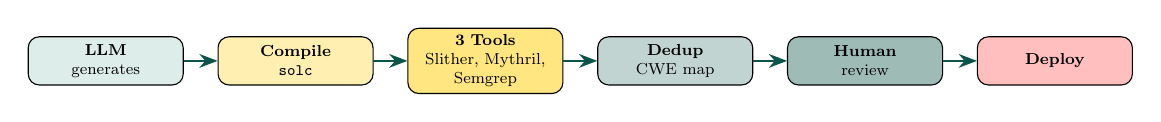
\begin{tikzpicture}[node distance=0.4cm, scale=0.72, transform shape]
    \node[draw, rounded corners, fill=wsulightgreen, text width=2.5cm, align=center, font=\footnotesize, minimum height=0.85cm] (gen) {\textbf{LLM}\\generates};
    \node[draw, rounded corners, fill=wsugold!30, text width=2.5cm, align=center, font=\footnotesize, minimum height=0.85cm, right=0.6cm of gen] (comp) {\textbf{Compile}\\\texttt{solc}};
    \node[draw, rounded corners, fill=wsugold!50, text width=2.5cm, align=center, font=\footnotesize, minimum height=0.85cm, right=0.6cm of comp] (multi) {\textbf{3 Tools}\\Slither, Mythril, Semgrep};
    \node[draw, rounded corners, fill=wsugreen!25, text width=2.5cm, align=center, font=\footnotesize, minimum height=0.85cm, right=0.6cm of multi] (dedup) {\textbf{Dedup}\\CWE map};
    \node[draw, rounded corners, fill=wsugreen!40, text width=2.5cm, align=center, font=\footnotesize, minimum height=0.85cm, right=0.6cm of dedup] (human) {\textbf{Human}\\review};
    \node[draw, rounded corners, fill=red!25, text width=2.5cm, align=center, font=\footnotesize\bfseries, minimum height=0.85cm, right=0.6cm of human] (deploy) {Deploy};

    \draw[-{Stealth}, thick, wsugreen] (gen) -- (comp);
    \draw[-{Stealth}, thick, wsugreen] (comp) -- (multi);
    \draw[-{Stealth}, thick, wsugreen] (multi) -- (dedup);
    \draw[-{Stealth}, thick, wsugreen] (dedup) -- (human);
    \draw[-{Stealth}, thick, wsugreen] (human) -- (deploy);
\end{tikzpicture}
\end{center}

\vspace{0.15cm}
\begin{columns}
\begin{column}{0.48\textwidth}
\textbf{Why each step:}
\begin{itemize}\small
    \item 35\% doesn't compile $\to$ gate first
    \item Tools disagree ($\rho \approx 0.13$) $\to$ use 3
    \item Logic bugs hide from tools $\to$ humans
\end{itemize}
\end{column}
\begin{column}{0.48\textwidth}
\textbf{What we measured (1,566 contracts):}
\begin{itemize}\small
    \item 3 tools: \textbf{100\%} coverage vs 93.9\% Slither-only
    \item Dedup: \textbf{23\%} reduction (3,133 $\to$ 2,410)
    \item Human step validated on baseline only
\end{itemize}
\end{column}
\end{columns}

\vspace{0.1cm}
{\scriptsize\textit{End-to-end precision/recall on a ground-truth corpus remains future work.}}
\end{frame}

%--- Slide 17: Contributions ---
\begin{frame}{Implications and Contributions}
\begin{columns}
\begin{column}{0.5\textwidth}
\textbf{For developers:}
\begin{enumerate}\small
    \item Never deploy without auditing
    \item Don't trust security prompts
    \item Prefer GPT-5
    \item Extra care: DeFi, long code
    \item Watch the second half
\end{enumerate}
\end{column}
\begin{column}{0.48\textwidth}
\textbf{Our contributions:}
\begin{enumerate}\small
    \item Largest study: 2,400 contracts, 8 LLMs
    \item Adversarial null result (new)
    \item 3 novel LLM patterns
    \item Root cause analysis
    \item Real Ethereum baseline + review
\end{enumerate}
\end{column}
\end{columns}
\end{frame}

%--- Slide 18: Limitations ---
\begin{frame}{Limitations and Future Work}
\begin{columns}
\begin{column}{0.48\textwidth}
\textbf{Limitations:}
\begin{itemize}\small
    \item Snapshot --- models change
    \item Static tools have false positives
    \item 8 LLMs, not all
    \item Solidity only
    \item Single-shot, no multi-turn
\end{itemize}
\end{column}
\begin{column}{0.48\textwidth}
\textbf{Future work:}
\begin{itemize}\small
    \item Rust/Solana, Move/Aptos
    \item Fuzzing, runtime analysis
    \item Multi-turn developer sessions
    \item LLM-aware static tools
    \item Security fine-tuning
\end{itemize}
\end{column}
\end{columns}
\end{frame}

%--- Slide 19: Summary + Thank You ---
\begin{frame}{Summary}
\begin{center}
\small
\begin{tabular}{@{}rl@{}}
\textbf{2,400} & contracts from 8 LLMs \\
\textbf{2,493} & unique bugs \\
\textbf{54.7\%} & of compiled have real bugs \\
\textbf{26.8\%} & have high-severity \\
\textbf{$p = 0.965$} & adversarial doesn't matter \\
\textbf{0.99--4.88} & LLM bugs per 100 LOC \\
\textbf{2.69} & human baseline density \\
\end{tabular}
\end{center}

\vspace{0.15cm}
\begin{block}{}
\centering
LLM code isn't worse than human code --- \\
but it skips the audit pipeline.
\end{block}

\vspace{0.2cm}
\begin{center}
{\large\bfseries Thank you! \quad Questions?}\\[0.2cm]
\small\texttt{github.com/atahabilder1/AiContractCheck}
\end{center}
\end{frame}

\end{document}
